%%%%%%%%%%%%%%%%%%%%%%%%%%%%%%%%%%%%%
\part{Preliminaries}
%%%%%%%%%%%%%%%%%%%%%%%%%%%%%%%%%%%%%

%%% --------------------------
\section{Motivation}
\subsection{Why tutorial?} 
%%% --------------------------
\normalfont
\begin{frame}
	\begin{center}
  		\begin{alertblock}{Why Tutorial?} 
  			\begin{itemize}
  				\item Derive and convey key insights from data
  				\item Learn and use open source software
  				\item Explore first/another programming language
  				\item Gain ability to create insightful visualizations
  				\item Be more marketable 
  			\end{itemize}
		\end{alertblock}

	       \begin{center}
	         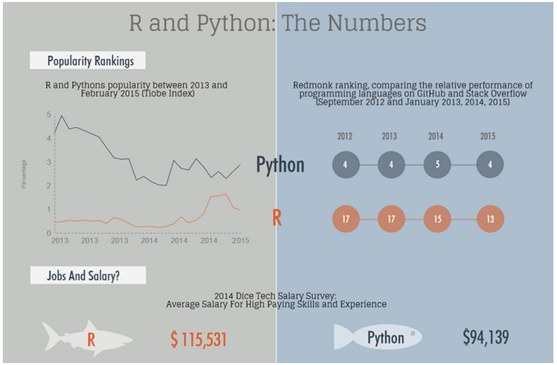
\includegraphics[scale=0.25]{images/r-vs-python-numbers}[6]
	        \end{center}

	\end{center} 
\end{frame}


%%% --------------------------
\subsection{Why R?}
%%% --------------------------
\begin{frame}
	\begin{center}
  		\begin{block}{Why R?} 
			\begin{itemize}
				\item Absolutely free!
				\item Used in industry and academia.
				\item Has a great community:
					\begin{itemize}
						\item StackOverflow
						\item Blogs
						\item Meetup groups
						\item MOOCs
						\item many, many others
					\end{itemize}
				\item Has over 7900 packages available for use (for free!).
				\item Transparent code (e.g. easier to check for bugs).
			\end{itemize}
		\end{block}
	\end{center} 
\end{frame}

%%% --------------------------
\subsection{Why visualize?}
%%% --------------------------
\begin{frame}
	\frametitle{Approach 1: Infographic}
	\begin{center}
		\vspace{-10pt}
  		\begin{block}{Inforgraphic} 
			\begin{itemize}
				\item Manually created
				\item Customized to a data set
				\item Art
			\end{itemize}
		\end{block}
	\end{center}	

   \begin{center}
     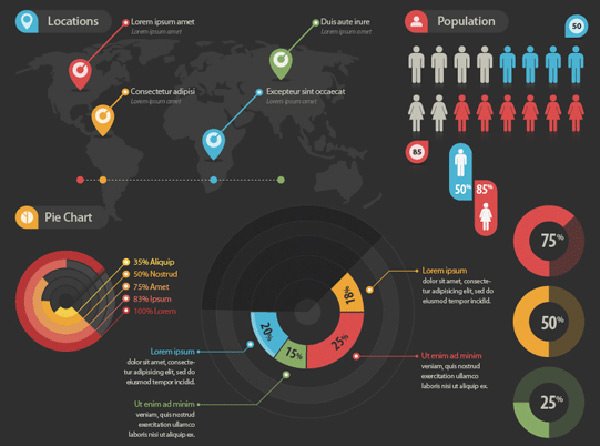
\includegraphics[scale=0.25]{images/infographic}[10]
    \end{center}

\end{frame}


\begin{frame}[allowframebreaks]
	\frametitle{Approach 2: Data Visualization}
  		\begin{block}{Data Visualization} 
			\begin{itemize}
				\item Automated via software
				\item Reproducible for a different data set
				\item (Less? of an) art
			\end{itemize}
		\end{block}
		There are two types of data visualization:
			\begin{block}{1. Exploratory} 
					\begin{itemize}
						\item \small Capture uncertainty in the data
						\item Explore potential relationships/trends/missing patterns (or absence thereof)
					\end{itemize}
			\end{block}
			\begin{block}{2. Explanatory}
					\begin{itemize}
						\item Convey key information \normalfont
					\end{itemize}
			\end{block}

   \begin{center}
     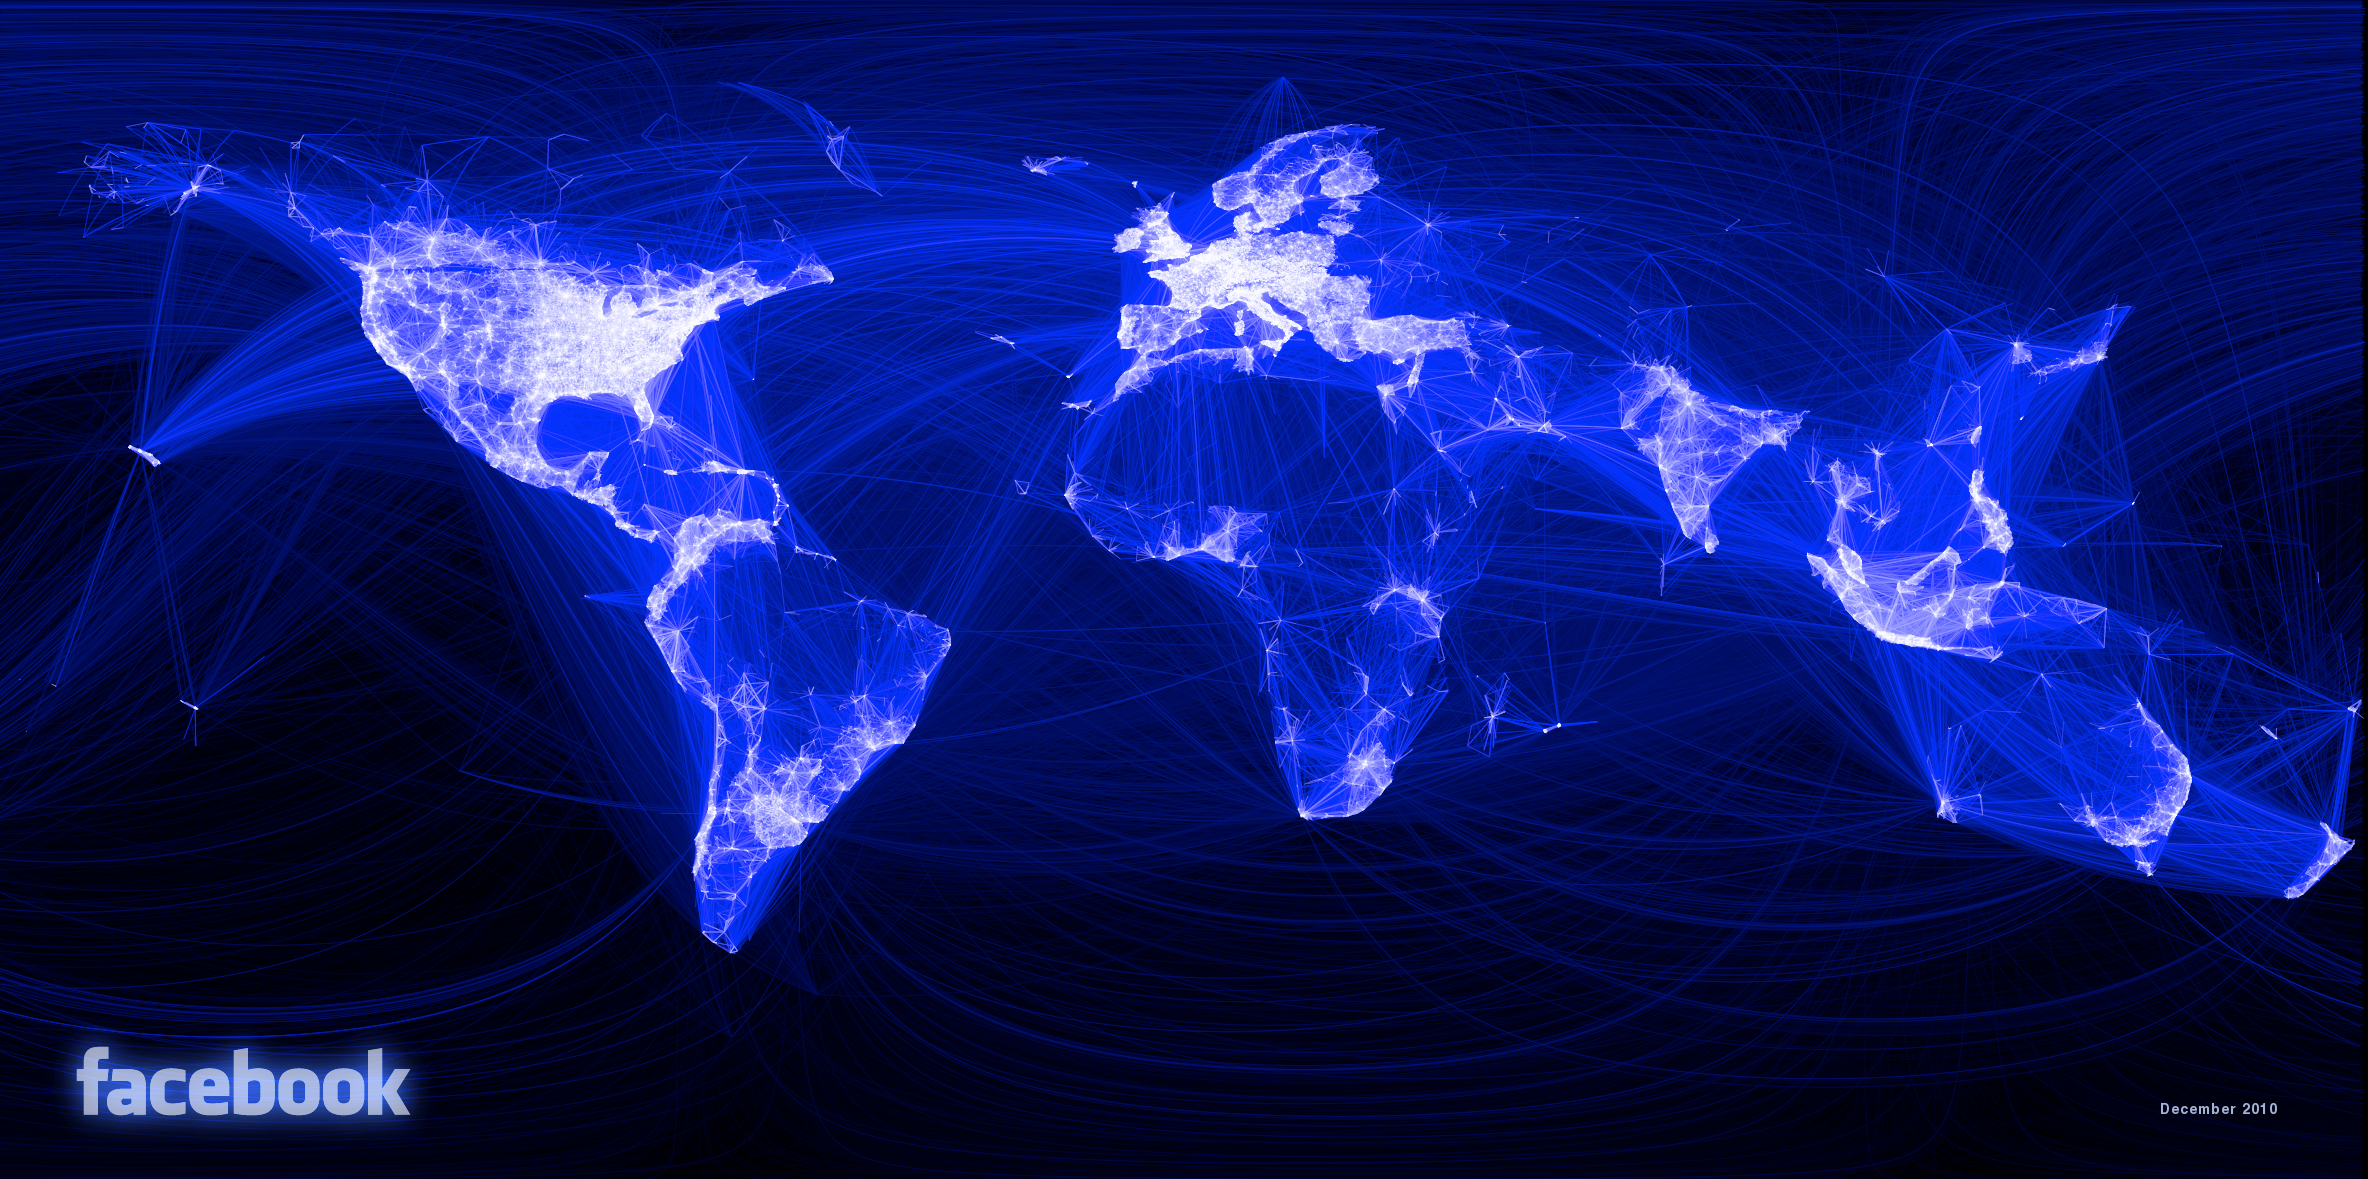
\includegraphics[scale=0.09]{images/facebook}[8]
    \end{center}

\end{frame}
%---

%%% --------------------------
\section{Tips for Visulizations}
%%% --------------------------
\begin{frame}
	\frametitle{Tips for visualizations} 
	\begin{itemize}
		\item Know your audience 
		\item \itshape{ 15 second rule:} \normalfont if your audience won't be able to understand the graphic in 15 seconds, simplify
		\item Layout [9] and font choices
		\item Color choices 
			\begin{itemize}
				\item Available colors in R: 
					\begin{itemize}
						\item \small{\url{http://research.stowers-institute.org/efg/R/Color/Chart/}} \normalfont
					\end{itemize}
				\item Color blindness simulation [11]:
					\begin{itemize}
						\item \url{http://vischeck.com}
						\item \url{http://rsb.info.nih.gov/ij/}
					\end{itemize}
			\end{itemize} 
		\item Add text/labels to figure
	\end{itemize}		


  % \begin{center}
  % 	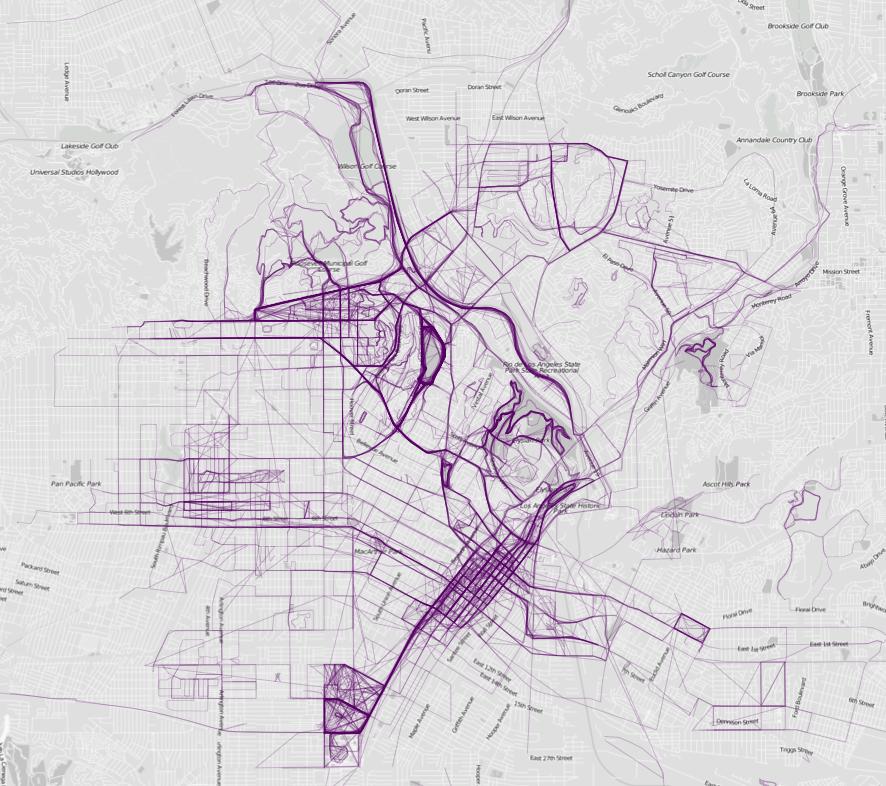
\includegraphics[width=0.4\textwidth]{images/geolocation_ex2}[7]
  % \end{center}

\end{frame}
%---




%%%%%%%%%%%%%%%%%%%%%%%%%%%%%%%%%%%%%
\part{Introduction to R}
%%%%%%%%%%%%%%%%%%%%%%%%%%%%%%%%%%%%%

%%% --------------------------
\section{Installing R and RStudio}
%%% --------------------------
\begin{frame}
  \frametitle{Installing R and RStudio}
  		\vspace{-5pt}
        \begin{enumerate}
           \item[R:] Go to \small \url{http://cran.r-project.org/}, select your operating system and download the latest version: 3.2.3 (Release 2015/12/10).
           \item[RStudio:] Go to \small \url{https://www.rstudio.com/products/rstudio/download/}, select your operating system and download the installer (if available).
        \end{enumerate}
%
		\vspace{-5pt}
       \begin{center}
         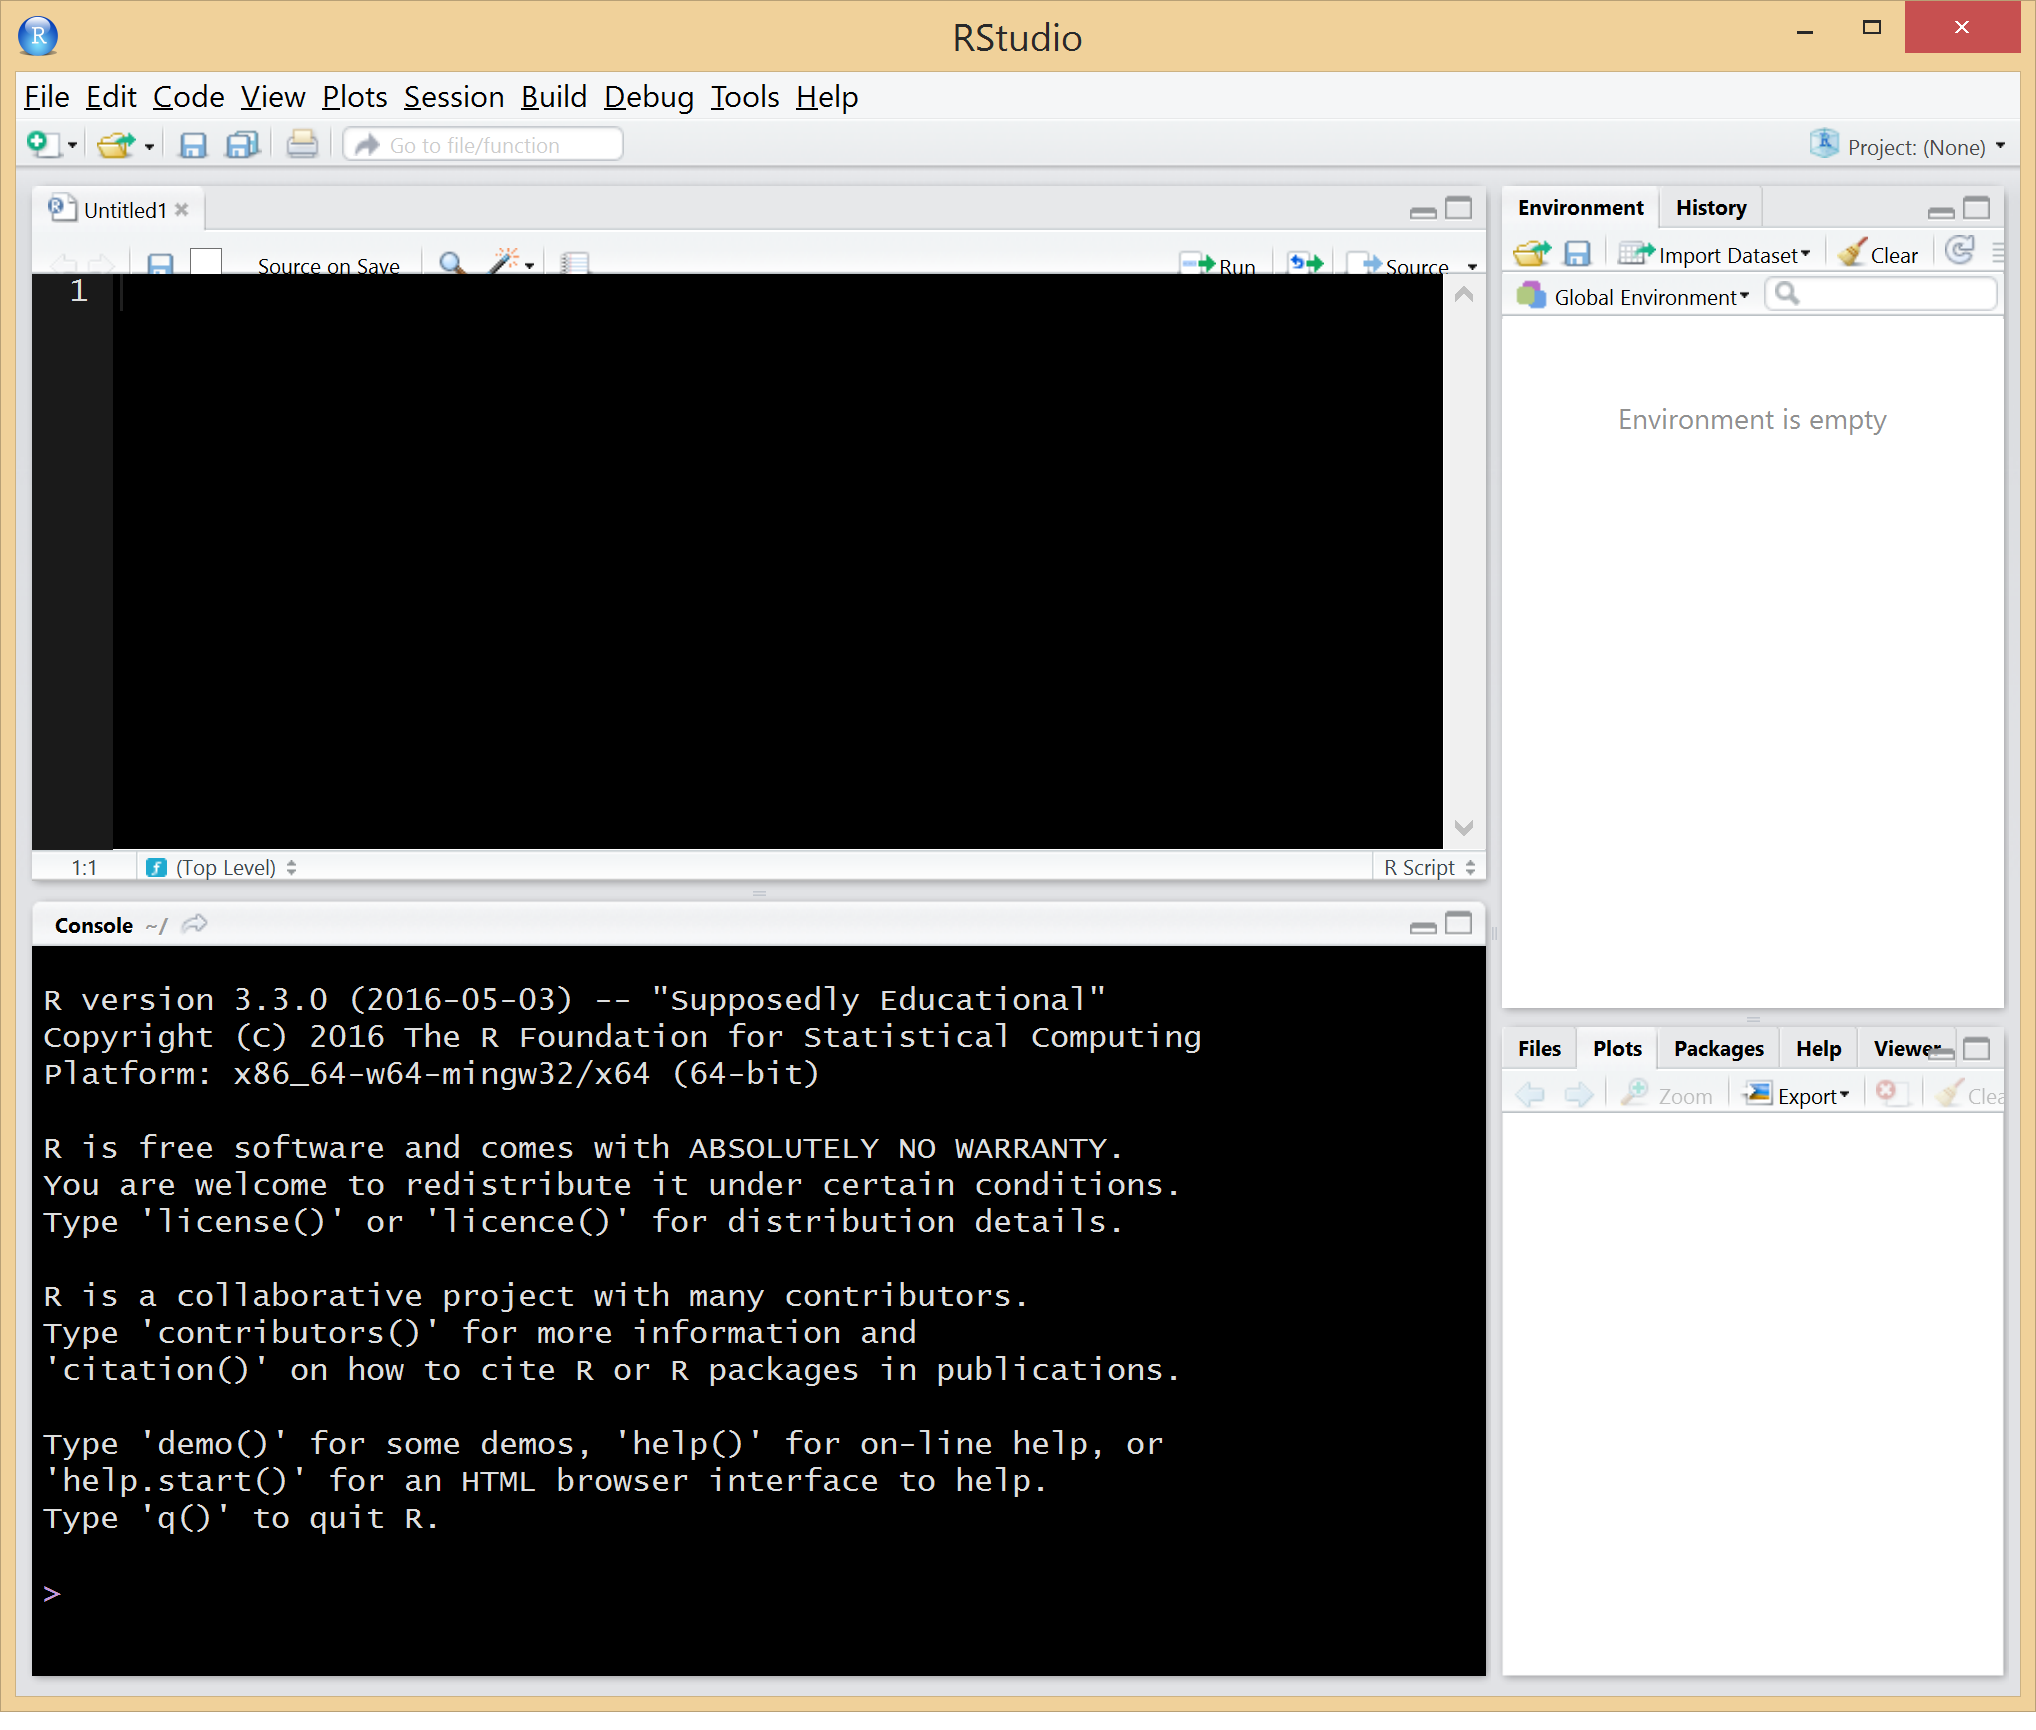
\includegraphics[width=0.5\textwidth]{images/Rwindow.png}
        \end{center}
\end{frame}


%%% --------------------------
\section{Overview of R}
%%% --------------------------
\begin{frame}
	\begin{center}
  		\begin{block}{Overview of R per John Chambers [1]:} 
			"To understand computations in R, two slogans are helpful:
			\begin{itemize}
			        \item Everything that exists is an object.
			        \item Everything that happens is a function call."
			\end{itemize}
		\end{block}
	\end{center} 

% R is flexible: 
% 	\begin{itemize}
% 		\item Objects can be variables, data sets, etc. and can be self-created, downloaded off the web (or elsewhere) and loaded from package(s).
% 		\item Functions (which do something to objects) can also be self-created, downloaded off the web (or elsewhere) and loaded from package(s).
% 		\item A package (1 of 7500+) is a collection of data sets and/or functions unified with a common theme.
% 	\end{itemize}
\end{frame}

%%% --------------------------
\subsection{Creating Objects}
%%% --------------------------
\begin{frame}[allowframebreaks]
	\frametitle{Objects in R}
		\begin{block}{Creating objects in R}
Objects can be created in different ways, via:
			\begin{itemize}
				\item equal sign: \lstinline$ x = 3 $
				\item left arrow: \lstinline$ y <- 2 * x + 1 $
				\item right arrow: \lstinline$ 10 -> z $
			\end{itemize}
		\end{block}

\newpage
	\begin{block}{Examples of Objects}
		\begin{itemize}
			\item[]
			\item Variables, which can be either discrete or continuous:
				\begin{itemize} 
					\item[Discrete:] e.g. number of people at the tutorial
					\item[Continuous:] e.g. how long it took to get to the tutorial
				\end{itemize}
			\item[]
			\item Data frames, which contain data sets with at least one variable:
				\begin{itemize} 
					\item[EX 1:] e.g. data set of commonly performed procedures at CA hospitals (variables include hospital name, procedure type, number of patients who had that procedure, etc.)
					\item[EX 2:] e.g. data set of popular movies (variables include movie name, genre, lead actor/actress, etc.)
				\end{itemize}
		\end{itemize}
	\end{block}

\end{frame}

%%% --------------------------
\subsection{(Very) Brief Overview of Functions}
%%% --------------------------
\begin{frame}[fragile]
	\frametitle{Functions in R}
	\vspace{-15pt}
	\begin{center}
		\begin{block}{Function by example}
			\begin{lstlisting}[ basicstyle=\tiny]
f <- function(x, y=1){
	answer <- x * 2 + y + 1
	return(answer)
}

f(2)        # 6
f(3, 2)     # 9
f(y=3, 2)   # 8
f(y=3, x=3) # 10
			\end{lstlisting}	
		\end{block}

		\vspace{-5pt}
		\begin{block}{Components of a function:}
			\begin{itemize}
				\item Assign function to a variable
				\item Add the 'function' keyword
				\item Specify arguments (if any) that function needs to compute result
				\item Specify any argument defaults
			\end{itemize}
					%%% Assignment, arguments, named, order, unnamed
		\end{block}
	\end{center} 
\end{frame}

%%% --------------------------
\subsection{Comparisons}
%%% --------------------------
\begin{frame}[fragile]
\frametitle{Making Comparisons}
Comparisons return a TRUE or FALSE depending on the condition evaluated:
			\begin{lstlisting}
# Suppose x and y are:
x = 3
y = 5
			\end{lstlisting}
			\begin{lstlisting}[ basicstyle=\footnotesize]
What should the following comparisons return?
x == 3  # is x 3?
x != y  # are x and y different?
x >= y  # is x greater than or equal to y?
(x==3) & (y==4) # is it true that x is 3 and y is 4?
(x==3) | (y==4) # is it true that x is 3 or y is 4?
			\end{lstlisting}	
\end{frame}

%%% --------------------------
\subsection{(More) Notation}
%%% --------------------------
\begin{frame}[fragile, allowframebreaks]
	\frametitle{Notation/Conventions}

	\vspace{10pt}
	\begin{itemize}
		\item[\%$>$\%:] 'pipe operator' which sends objects on the left-hand side to be processed by functions on the right-hand side [15]
			\begin{itemize}
				\item x \%$>$\% f is equivalent to f(x)
			\end{itemize}
		\item[c():] 'concatenation' which combines objects together
			\begin{lstlisting}
x = 3
y = 5
z = c(x, y) 
z
			\end{lstlisting}
			\begin{verbatim}
[1] 3 5
			\end{verbatim}
		\end{itemize}

\newpage
	\begin{itemize}		
		\item[Brackets:] 'subsetting' which says what observation we are (not) interested in
			\begin{lstlisting}
# Example 1:
z = c(3, 5) 
z[2]
			\end{lstlisting}
			\begin{verbatim}
[1] 5
			\end{verbatim}		
			\begin{lstlisting}
# Example 2:
z = c(3, 5) 
z[ z > 3 ]
			\end{lstlisting}
			\begin{verbatim}
[1] 5
			\end{verbatim}						
	\end{itemize}

\end{frame}


\section{Working with Data}

\subsection{Reading Data from File}

%%%%%%%%%%%%%%%%%%%%%%%%%%%%%%%%%%%%%
% --------------------------------------------------- Slide --
\begin{frame}[fragile, allowframebreaks]
 \frametitle{Reading Data from File}

One approach is via \ttfamily read.table(). \normalfont  In the arguments of the function:
  \begin{itemize}
  \item \ttfamily file: \normalfont specifies the (relative) location, file name and file extension
  \item \ttfamily header: \normalfont if TRUE, tells R to include variables names when importing
  \item \ttfamily sep: \normalfont tells R how the entires in the data set are separated
    \begin{itemize}
      \item \ttfamily sep=",": \normalfont when entries are separated by COMMAS
      \item \ttfamily sep="$\backslash t$":\normalfont \hspace{2.5pt} when entries are separated by TAB
      \item \ttfamily sep=" ": \normalfont when entries are separated by SPACE
    \end{itemize}
   \end{itemize}

\newpage   
   	\begin{lstlisting}[ basicstyle=\footnotesize]
filepath = "http://www.ats.ucla.edu/stat/data/test_missing_comma.txt"
### Other valid paths:
# filepath = "C:/Documents/test_missing_comma.txt"
# filepath = "./test_missing_comma.txt"

df <- read.table(
	file = filepath, 
	header = TRUE, 
	sep = ","
	)
	\end{lstlisting}
\normalfont
\normalsize
\end{frame}

%%% --------------------------
\subsection{Working with Data Frames}
%%% --------------------------
\begin{frame}[fragile, allowframebreaks]
	\frametitle{Working with Data Frames}
	To check that a data set has been read-in correctly: 
	\begin{itemize}
		\item View the complete data set by typing the variable name.  (This is not recommended for large data sets.) 
\begin{lstlisting}
df
\end{lstlisting}

{ \small
\begin{verbatim}
    prgtype gender  id ses schtyp level
1   general      0  70   4      1     1
2    vocati      1 121   4     NA     1
3   general      0  86  NA     NA     1
4    vocati      0 141   4      3     1
5  academic      0 172   4      2     1
6  academic      0 113   4      2     1
7   general      0  50   3      2     1
8  academic      0  11   1      2     1
\end{verbatim}
}

\newpage		
		\item View the first 5 lines of the dataset via \ttfamily head(): \normalfont 
\begin{lstlisting}
head(df, 5) 
\end{lstlisting}

\begin{verbatim}
    prgtype gender  id ses schtyp level
1   general      0  70   4      1     1
2    vocati      1 121   4     NA     1
3   general      0  86  NA     NA     1
4    vocati      0 141   4      3     1
5  academic      0 172   4      2     1
\end{verbatim}

\newpage
		\item View the last 7 lines of the dataset via \ttfamily tail(): \normalfont 
\begin{lstlisting}
tail(df, 7)
\end{lstlisting}

\begin{verbatim}
    prgtype gender  id ses schtyp level
2    vocati      1 121   4     NA     1
3   general      0  86  NA     NA     1
4    vocati      0 141   4      3     1
5  academic      0 172   4      2     1
6  academic      0 113   4      2     1
7   general      0  50   3      2     1
8  academic      0  11   1      2     1
\end{verbatim}		

\newpage
		\item Check the variable names via \ttfamily names(): \normalfont 
\begin{lstlisting}
names(df)
\end{lstlisting}

{ \footnotesize
	\begin{verbatim}
[1] "prgtype" "gender"  "id"      "ses"     "schtyp"  "level"
	\end{verbatim}
}	
		\item Check the size of the data set via \ttfamily dim(): \normalfont 
\begin{lstlisting}
dim(df)
\end{lstlisting}

\begin{verbatim}
[1] 8 6
\end{verbatim}	
		\item See the first 3 entries for variable 'gender' via \ttfamily head(): \normalfont 
\begin{lstlisting}
head(df$gender)
\end{lstlisting}

\begin{verbatim}
[1] 0 1 0 0 0 0
\end{verbatim}	

\newpage
	\item Examine how many unique levels a variable has via \ttfamily unique(): \normalfont
\begin{lstlisting}
unique(df$gender)
\end{lstlisting}

\begin{verbatim}
[1] 0 1
\end{verbatim}	
	\item Examine the counts of levels that a variable has via \ttfamily table(): \normalfont
\begin{lstlisting}
table(df$gender, useNA='always')
\end{lstlisting}

\begin{verbatim}
   0    1 <NA> 
   7    1    0 
\end{verbatim}	

\newpage
		\item Verify ranges and check for missing data via \ttfamily summary(): \normalfont 
\begin{lstlisting}
summary(df)
\end{lstlisting}

{ \tiny
	\begin{verbatim}
      prgtype      gender            id             ses            schtyp      level  
    vocati:2   Min.   :0.000   Min.   : 11.0   Min.   :1.000   Min.   :1   Min.   :1  
   general:3   1st Qu.:0.000   1st Qu.: 65.0   1st Qu.:3.500   1st Qu.:2   1st Qu.:1  
  academic:3   Median :0.000   Median : 99.5   Median :4.000   Median :2   Median :1  
               Mean   :0.125   Mean   : 95.5   Mean   :3.429   Mean   :2   Mean   :1  
               3rd Qu.:0.000   3rd Qu.:126.0   3rd Qu.:4.000   3rd Qu.:2   3rd Qu.:1  
               Max.   :1.000   Max.   :172.0   Max.   :4.000   Max.   :3   Max.   :1  
                                               NA's   :1       NA's   :2              
	\end{verbatim}	
}
	\end{itemize}
\end{frame}


%%% --------------------------
\section{Adding Functionality to Base R}
%%% --------------------------

\begin{frame}[fragile]
	\frametitle{Adding Functionality to Base R}

	\begin{itemize}
		\item Base R is what you download off CRAN \url{www.cran.r-project.org} 
		\item Available packages are listed here: \url{https://cran.r-project.org/web/packages/}
		\item Install an R package(s) via \ttfamily install.packages(): \normalfont 
   	\begin{lstlisting}[ basicstyle=\small]
install.packages("lattice")
install.packages("ggplot2")
# OR
install.packages( c("lattice", "ggplot2") )

	\end{lstlisting}
	\end{itemize} 	
\end{frame}



%%%%%%%%%%%%%%%%%%%%%%%%%%%%%%%%%%%%%
